\section{Solution}
The mean reversion method was first proposed by Lo \emph{et al.}\cite{mean_reverse} in 1990. The basic idea is that better performing stocks tend to perform worse than others in the subsequent trading days, and the worse performing stocks are inclined to perform better. Thus to maximize the portfolio return for the next trading day, we can minimize the expected portfolio return with respect to today's price relative since the next price relative tends to revert.  

The CWMR method models the portfolio vector for the $i$th trading day as a Gaussian distribution with mean $\mu\in \textbf{R}^m$ and the diagonal covariance matrix $\Sigma\in \textbf{R}^{m\times m}$ with nonzero diagonal elements $\sigma^2$.  The value $\mu_j$ represents the knowledge of stock $j$ in the portfolio.The diagonal covariance matrix term $\sigma_j^2$ stands for the confidence we have in the portfolio mean value $\mu_j$.  In this case, the authors not only exploit the first order information (mean) of the portfolio, but also combine the second order information of the portfolio (volatility).

Since $\textbf{b}_i \sim \mathcal{N}(\mu, \Sigma)$, and  $\textbf{s}_i = \textbf{b}_i^T x_i$, the daily portfolio return also follows Gaussian distribution: $\textbf{s}_i \sim \mathcal{N}(\mu\cdot x_i, x_i^T\Sigma x_i)$.

If the expected portfolio return using the $i$th price relative is less than a threshold with high probability, the actual return for the $i+1$th trading day tends to be high with correspondingly high probability, since the price relative tends to reverse. Though we are more interested in the stocks with poor performance in the current trading day, we still would like to choose a Gaussian distribution as close to the current distribution $\mathcal{N}(\mu_i,\Sigma_i)$ as possible in the KL divergence sense. Passively choosing the closest distribution alleviates the fluctuation and ensures relatively good performance. On the $i+1$th trading day, the algorithm sets the parameters of the distribution by solving the following optimization problem:

\begin{equation}
\begin{split}
(\mu_{i+1}, \Sigma_{i+1}) &=\argmin_{\mu,\Sigma}~D_{KL}(\mathcal{N}(\mu,\Sigma) || \mathcal{N}(\mu_i,\Sigma_i))\\
& s.t.~ ~\textrm{Pr}[\mu\cdot x_i \le \epsilon] \ge \theta\\
& ~~~~~~~~\mu \in \Delta_m,
\label{eq:orginalOPT}
\end{split}
\end{equation}
The constraint ensures that expected portfolio return using the $i$th price relative is less than a threshold $\epsilon$ with probability larger than $\theta$. $\epsilon$ denotes the mean reversion threshold, and $\theta \in [0,1]$ represents the confidence level of the mean reversion. The constraint intrinsically models the fact that the chosen portfolio has high expectation to have low daily return in current trading day, and potentially has high return in the next trading day.

The combination of the the KL divergence and the constraint follows the idea of Passive Aggressive algorithm\cite{Crammer:2006:OPA:1248547.1248566}. The method is considered aggressive since it may aggressively approach a new portfolio if the constraint condition is no longer fulfilled, i.e., when the current portfolio brings in a high return. On the other hand, it also has a passive character because it will passively keep the current portfolio if the current portfolio keeps having poor performance.

A slight modification is made to the constraint so that it is now convex in covariance: $\epsilon - \log(\mu\cdot x_i) \ge \phi||\Upsilon x_i||$,
where $\Sigma = \Upsilon^2$, $\phi = \Phi^{-1}(\theta)$ and $\Upsilon$ is PSD. The solution to the optimization problem is expressed as:
\begin{equation}
\mu_{i+1} = \mu_{i} - \lambda_{i+1}\Sigma_i\bigg(\frac{x_i-\bar{x}_i\textbf{1}}{\mu_i\cdot x_i}\bigg), ~~~~~~\Sigma_{i+1}^{-1} = \Sigma_i^{-1} + \lambda_{i+1}\phi \frac{x_ix_i^T}{\sqrt{U_i}},
\label{eq:CWMR_update}
\end{equation}
 where $\sqrt{U_i} = \frac{-\lambda_{i+1} V_i\phi+ \sqrt{\lambda_{i+1}^2V_i^2\phi^2 +4V_i} }{2}$ and $V_i = x_i^T\Sigma_ix_i$. $\bar{x_i} = \frac{\textbf{1}^T \Sigma_i x_i}{\textbf{1}^T\Sigma_i \textbf{1}}$ represents the confidence weighted average of the $i$th price relative, and  $\lambda_{i+1}$ denotes the Lagrangian multiplier. Using KKT conditions similar as what we learned in SVM and applying Woodbury equation, we can derive the exact value of $\lambda$.
  
The mean $\mu_1$ and covariance matrix $\Sigma_1$ of portfolio is initialized to be $\frac{1}{m}\textbf{1}$ and $\frac{1}{m^2}\textbf{I}$, correspondingly. Everyday we update the portfolio distribution by updating the mean and covariance matrix according to Eq.~\ref{eq:CWMR_update}. The mean of portfolio is then projected to simplex domain to obtain the required portfolio.

\begin{figure}
%\centering
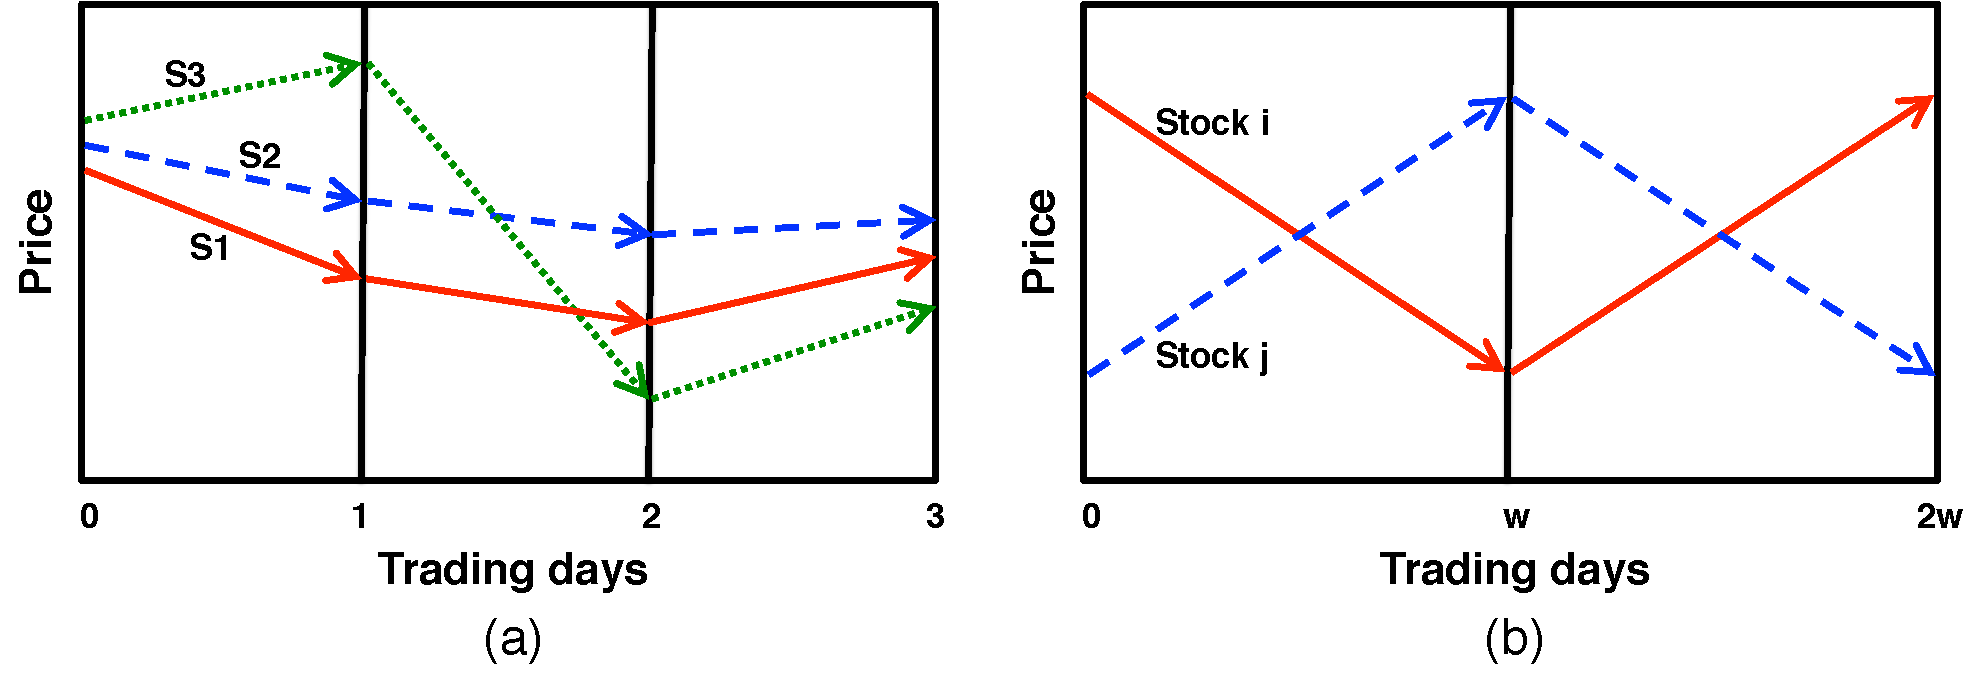
\includegraphics[width=\columnwidth]{illustration}
\caption{
\label{fig:illustration}
Two hypothetical stock charts for the illustration of CWMR and Anticor methods. (a) The price changes of three stocks in three trading days. CWMR assign weights to each stock based on their performance in the current trading day; (b) The price changes of stocks $i$ and $j$ over two consecutive windows with length of $w$ days. Anticor transfers investment from the well-performing stock to the anti-correlated poorly-performing stock.
}
\end{figure}

Let's look at one example on applying CWMR algorithm to three hypothetical stocks S1, S2, and S3 (FIG.~\ref{fig:illustration}(a)). Without any information of the market behavior prior to day 0, we first set the portfolio to be (1/3, 1/3, 1/3), with all the money equally distributed to the three stocks. When it comes to Day 1, we find S1 has the most poor performance so the portfolio may evolve to (1/2, 1/4, 1/4) to fulfill the constraint condition. On Day 2, we notice a big drop of S3, but we do not necessarily have to put more proportion of money on S3 as long as the current portfolio still has a poor performance. Therefore, we may still passively stick to the portfolio of (1/2, 1/4, 1/4). On Day 3, all the stocks rise so there is no way to find a positive portfolio that meet the requirement of the constraint. In that case, we project the calculated portfolio (probably negative) to the simplex domain for a positive portfolio with the smallest return.

The CWMR method does produce a huge return as we will present in the Evaluation section, but it was also pointed out in the paper that the cumulative wealth in the end is very sensitive to the ratio of transaction cost to the money invested. It has been shown that a transaction cost ratio as low as 0.8\% may reduce the final return from $10^{18}$\% to almost zero. This is understandable since CWMR requires trading tens of stocks everyday, and such a large basis of stocks was found necessary to guarantee a considerable amount of return. For this reason, this method may be feasible for large financial institutions, but not for personal investments.

Here we propose a revised method named ``A-Stock-A-Day Confidence Weighted Mean Reversion" (ASAD-CWMR). The idea is we only trade one stock a day though we keep a basis of tens or hundreds of stocks. While we update the portfolio distribution in exactly the same way as in CWMR, we only trade one stock from the portfolio everyday instead of all the stocks with positive components in the portfolio. We select this specific stock by ranking the portfolio components from highest to lowest, and take the first one that has negative performance in the current trading day. It takes much less transaction cost for ASAD-CWMR than for CWMR, and thus make it possible to apply the method even for personal investments. ASAD-CWMR is also more aggressive than the original CWMR method, since it only trades the stock with the highest weight, which is usually (but not always) one of those stocks that have the poorest performance in the current trading day. Every option has its pros and cons. As we will show in the Evaluation section, though ASAD-CWMR leads to higher return in certain periods of time, it has very poor performance during the time when the pattern of mean reversion is not very clear.
 
